\subsection{Etching With Acid:}

Ferric chloride is a common choice for an etchant ( this is the one that we use ). However, we can use Ammonium Persulfate crystals or other chemical solutions as we can see in Figure 3.4.0. No matter what choice for the chemical etchant, it will always be a dangerous material, so we need to be careful. \hfill \break

\begin{figure}[H]
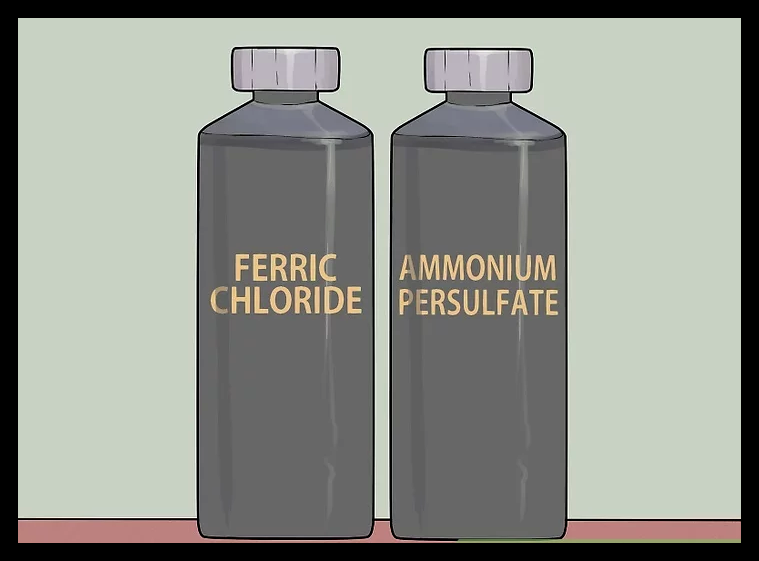
\includegraphics[height = 8cm, width = 16.5cm]{8.png}
\centering \linebreak \linebreak {\small Figure 3.4.0: Acids for Etching.}
\end{figure} \hfill \break

Depending on the acid etch that we choose, there might be additional instructions. For example, some crystallized acids require being dissolved in hot water, but other etchants are ready to use. So, ones the acid were prepared, we submerge the board in it as in Figure 3.4.1 and we make sure to stir every 3 or 5 minutes like in Figure 3.4.2.\hfill \break

\begin{figure}[H]
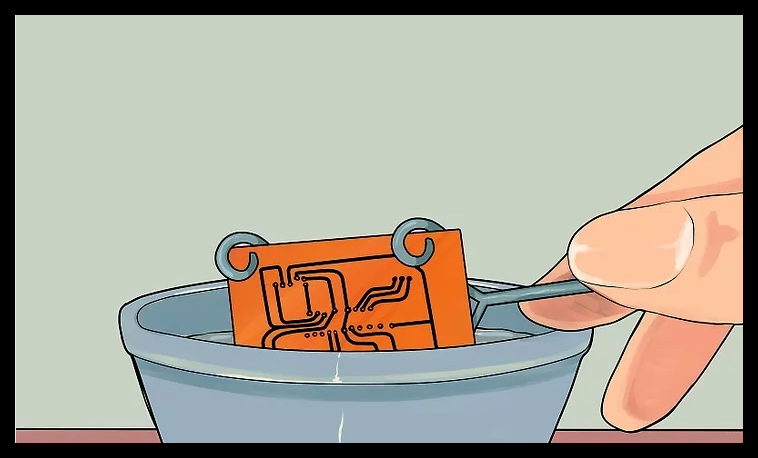
\includegraphics[height = 8cm, width = 16.5cm]{11.png}
\centering \linebreak \linebreak {\small Figure 3.4.1: Submerging the board.}
\end{figure} \hfill \break

\begin{figure}[H]
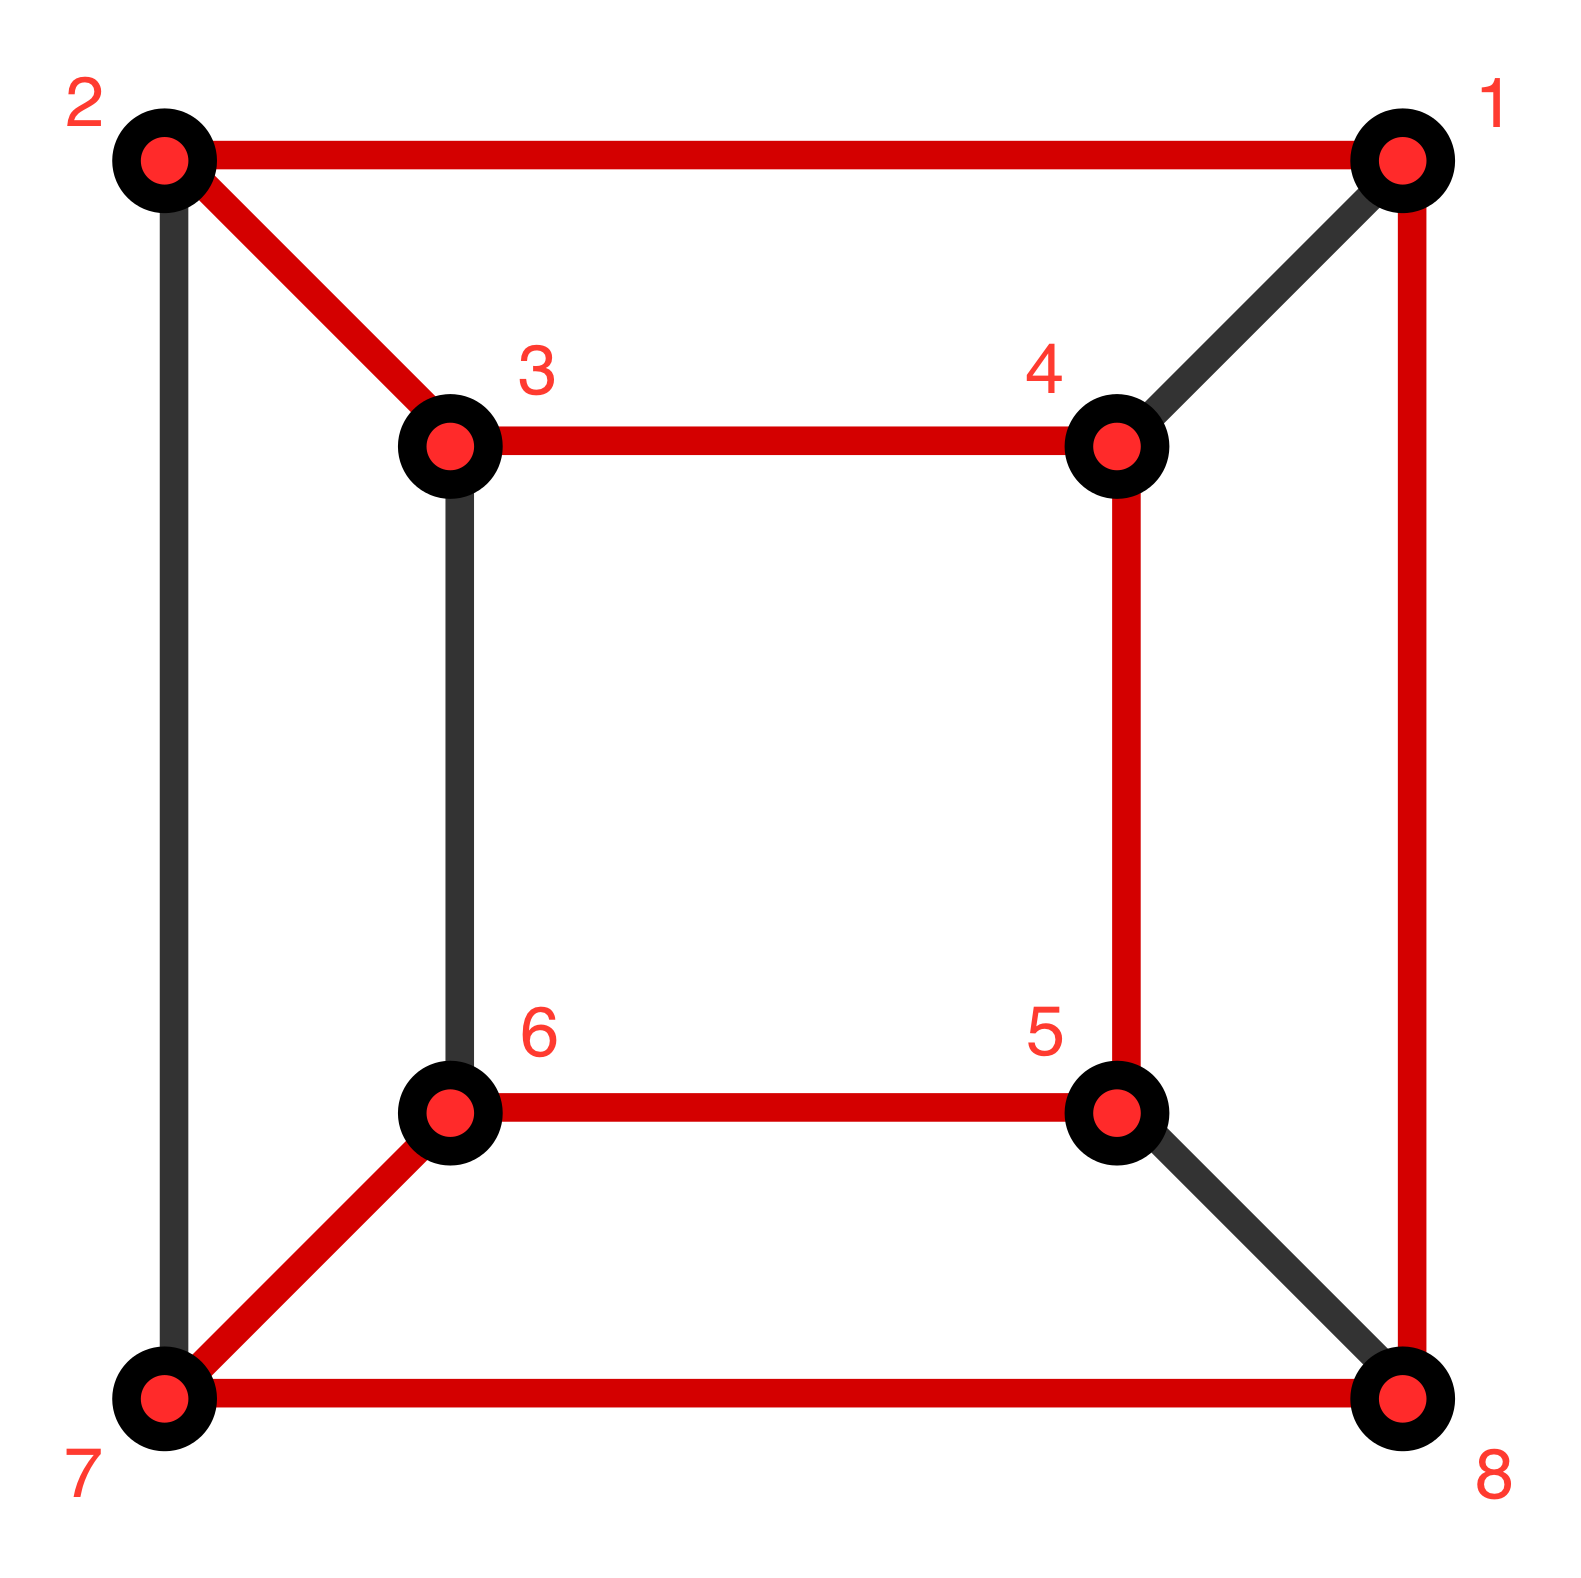
\includegraphics[height = 8cm, width = 16.5cm]{12.png}
\centering \linebreak \linebreak {\small Figure 3.4.2: Stir every 3-5 minutes.}
\end{figure}

\pagebreak

In Figure 3.4.3 we already submerge our circuit board. \hfill \break

\begin{figure}[H]
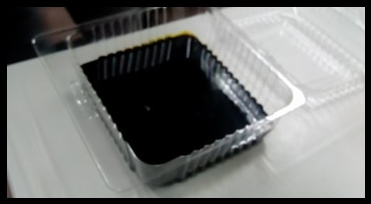
\includegraphics[height = 8cm, width = 16.5cm]{2c.jpg}
\centering \linebreak \linebreak {\small Figure 3.4.3: Circuit board submerged.}
\end{figure} \hfill \break

Finally, we take the board out and wash it when all unnecessary copper is etched away from the board ( Figure 3.4.4 ). \hfill \break

\begin{figure}[H]
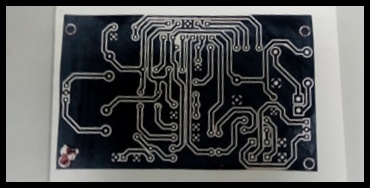
\includegraphics[height = 8cm, width = 16.5cm]{2a.jpg}
\centering \linebreak \linebreak {\small Figure 3.4.4: Circuit board cleaned after taked it out of the acid.}
\end{figure}

\pagebreak

There are special solvents available for almost all types of insulating drawing material used in drawing PCB layouts. However, we use sandpaper and our PCB it's finish as we can see in Figure 3.4.5. \hfill \break

\begin{figure}[H]
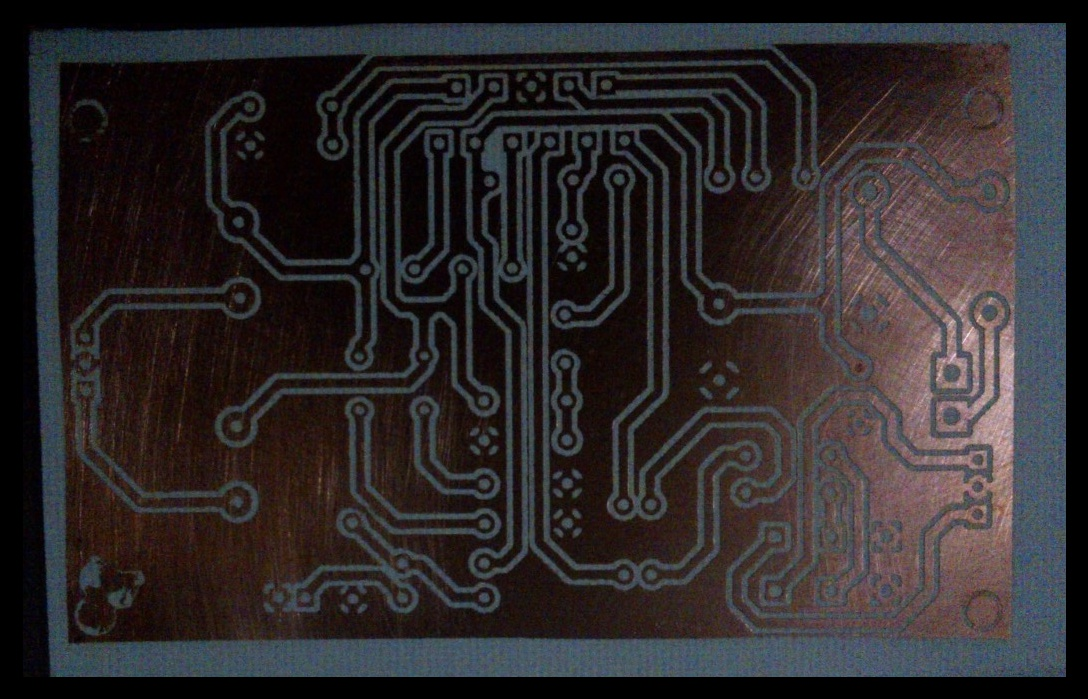
\includegraphics[height = 8cm, width = 16.5cm]{3a.jpg}
\centering \linebreak \linebreak {\small Figure 3.3.5: PCB finished.}
\end{figure} 

\pagebreak